% Options for packages loaded elsewhere
\PassOptionsToPackage{unicode}{hyperref}
\PassOptionsToPackage{hyphens}{url}
%
\documentclass[
]{book}
\usepackage{amsmath,amssymb}
\usepackage{iftex}
\ifPDFTeX
  \usepackage[T1]{fontenc}
  \usepackage[utf8]{inputenc}
  \usepackage{textcomp} % provide euro and other symbols
\else % if luatex or xetex
  \usepackage{unicode-math} % this also loads fontspec
  \defaultfontfeatures{Scale=MatchLowercase}
  \defaultfontfeatures[\rmfamily]{Ligatures=TeX,Scale=1}
\fi
\usepackage{lmodern}
\ifPDFTeX\else
  % xetex/luatex font selection
\fi
% Use upquote if available, for straight quotes in verbatim environments
\IfFileExists{upquote.sty}{\usepackage{upquote}}{}
\IfFileExists{microtype.sty}{% use microtype if available
  \usepackage[]{microtype}
  \UseMicrotypeSet[protrusion]{basicmath} % disable protrusion for tt fonts
}{}
\makeatletter
\@ifundefined{KOMAClassName}{% if non-KOMA class
  \IfFileExists{parskip.sty}{%
    \usepackage{parskip}
  }{% else
    \setlength{\parindent}{0pt}
    \setlength{\parskip}{6pt plus 2pt minus 1pt}}
}{% if KOMA class
  \KOMAoptions{parskip=half}}
\makeatother
\usepackage{xcolor}
\usepackage{longtable,booktabs,array}
\usepackage{calc} % for calculating minipage widths
% Correct order of tables after \paragraph or \subparagraph
\usepackage{etoolbox}
\makeatletter
\patchcmd\longtable{\par}{\if@noskipsec\mbox{}\fi\par}{}{}
\makeatother
% Allow footnotes in longtable head/foot
\IfFileExists{footnotehyper.sty}{\usepackage{footnotehyper}}{\usepackage{footnote}}
\makesavenoteenv{longtable}
\usepackage{graphicx}
\makeatletter
\def\maxwidth{\ifdim\Gin@nat@width>\linewidth\linewidth\else\Gin@nat@width\fi}
\def\maxheight{\ifdim\Gin@nat@height>\textheight\textheight\else\Gin@nat@height\fi}
\makeatother
% Scale images if necessary, so that they will not overflow the page
% margins by default, and it is still possible to overwrite the defaults
% using explicit options in \includegraphics[width, height, ...]{}
\setkeys{Gin}{width=\maxwidth,height=\maxheight,keepaspectratio}
% Set default figure placement to htbp
\makeatletter
\def\fps@figure{htbp}
\makeatother
\setlength{\emergencystretch}{3em} % prevent overfull lines
\providecommand{\tightlist}{%
  \setlength{\itemsep}{0pt}\setlength{\parskip}{0pt}}
\setcounter{secnumdepth}{5}
\usepackage{booktabs}
\ifLuaTeX
  \usepackage{selnolig}  % disable illegal ligatures
\fi
\usepackage[]{natbib}
\bibliographystyle{apalike}
\IfFileExists{bookmark.sty}{\usepackage{bookmark}}{\usepackage{hyperref}}
\IfFileExists{xurl.sty}{\usepackage{xurl}}{} % add URL line breaks if available
\urlstyle{same}
\hypersetup{
  pdftitle={Acute Pain Ketamine Guideline},
  pdfauthor={Lydia},
  hidelinks,
  pdfcreator={LaTeX via pandoc}}

\title{Acute Pain Ketamine Guideline}
\author{Lydia}
\date{2023-10-17}

\begin{document}
\maketitle

{
\setcounter{tocdepth}{1}
\tableofcontents
}
\hypertarget{summary}{%
\chapter{Summary}\label{summary}}

This document provides guidance on the dosing and administration of \textbf{low-dose ketamine} for \textbf{adults} with \textbf{uncontrolled} and \textbf{complex acute pain}.\citep{Brinck_2018} Low-dose ketamine should only be initiated, prescribed, titrated and discontinued by an acute pain consultant, anaesthetist and specialist pain nurses. This guideline does not cover the administration of ketamine as an anaesthetic agent or for the relief of procedural pain for areas such as the emergency department, and for chronic pain or palliative care.

\hypertarget{introduction}{%
\chapter{Introduction}\label{introduction}}

Acute pain is a common condition that requires effective and timely management to alleviate suffering and promote patient comfort, but also to prevent to development of chronic and persistent pain \citep{Brinck_2018}.

Some patients are thought to be at greater risk of developing persistent post-surgical pain for example, amputations, multiple fractures and polytrauma, which can be due to uncontrolled pre and post-operative pain and nerve damage \citep{Bell_2005}. The stress response, coupled with nerve damage can lead to wind-up and make controlling pain more difficult \citep{Mathew_2014}.

While opioids have traditionally been the mainstay of acute pain management, concerns regarding their adverse effects, escalating opioid requirements and the potential for dependence and misuse, has led to a search for alternative analgesic strategies \citep{Eipe_2018}.

Ketamine is an anaesthetic agent, but in low doses can be effective as an analgesic \textbf{without} inducing anaesthesia.

\begin{figure}
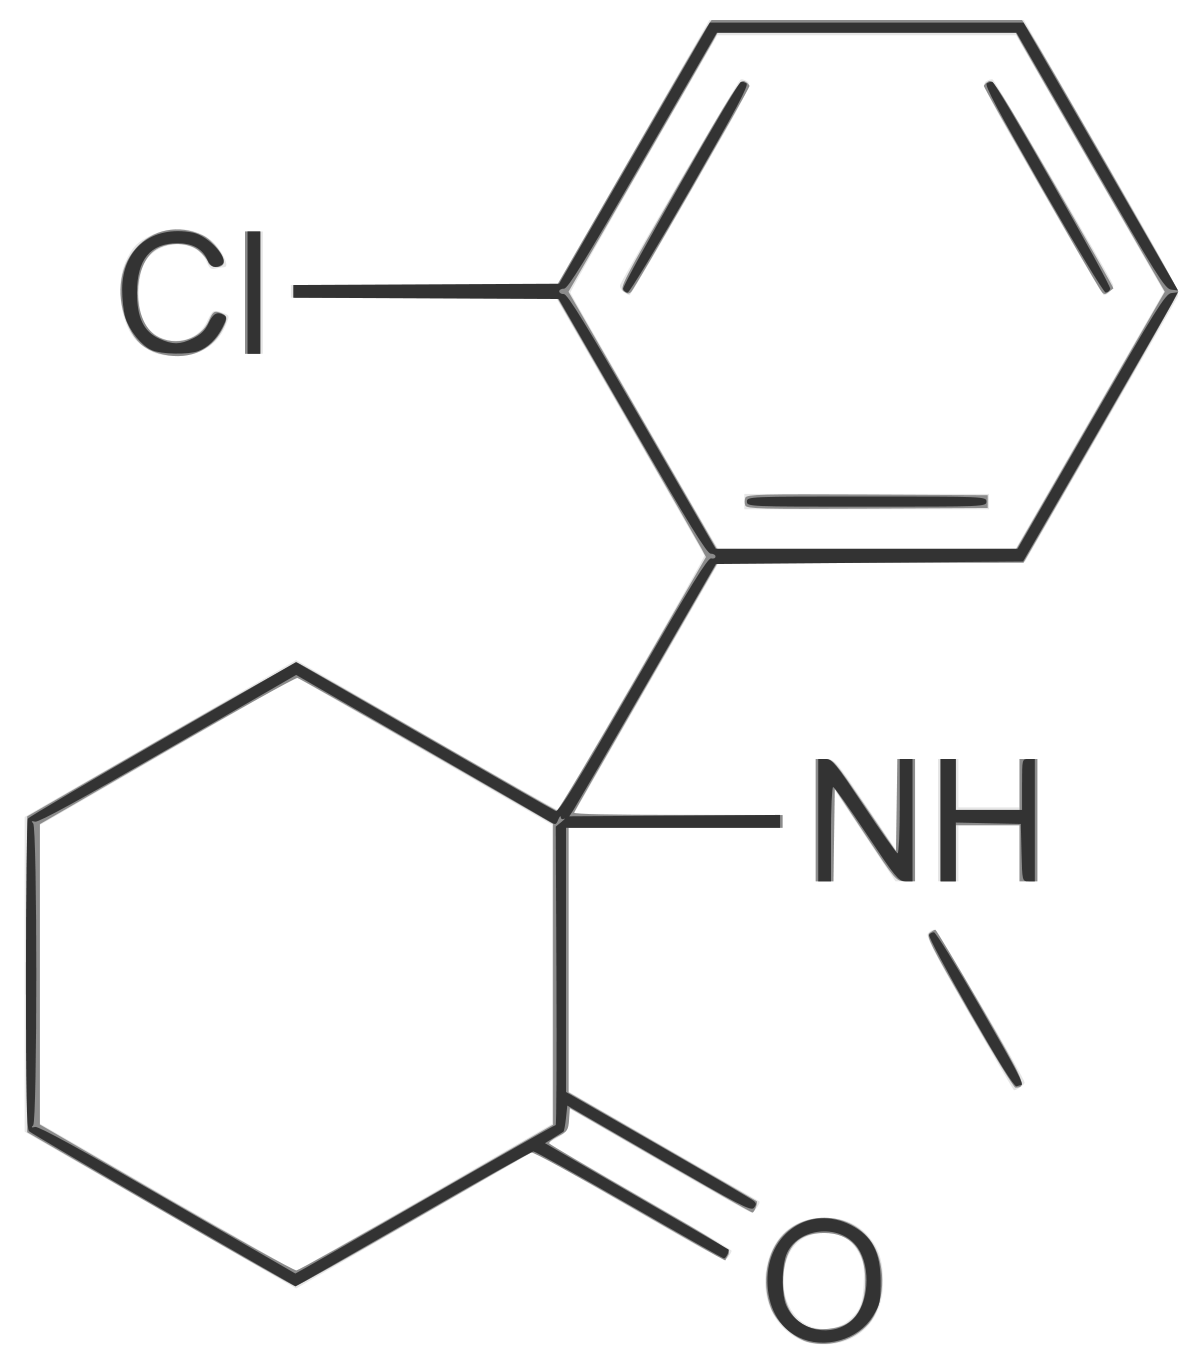
\includegraphics[width=0.7\linewidth]{ket_molecule} \caption{Ketamine (a phencyclidine derivative) is a N-methyl-D-aspartate receptor antagonists and dissociative analgesic and anesthetic.}\label{fig:unnamed-chunk-1}
\end{figure}

Ketamine works by blocking the \emph{N-methyl D-asparate} (NDMA) receptor, the receptor that is responsible of \textbf{amplifying pain signals}, the development of central sensitisation with opioid tolerance. This analgesic action occurs in the dorsal horn of the spinal cord, by reducing the action of glutamate -- the major excitatory neurotransmitter.\citep{magPain}

\begin{figure}
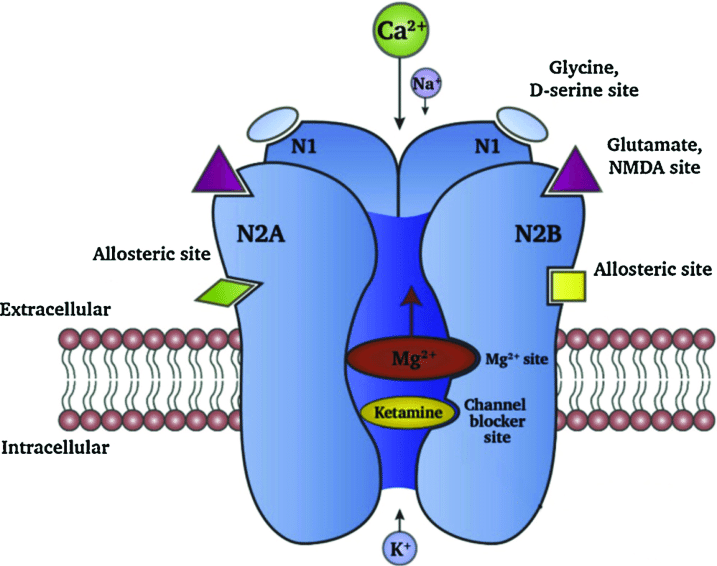
\includegraphics[width=0.7\linewidth]{NMDA} \caption{Diagram of the NMDA Receptor and Its Sites for Ligand Attachment: The NMDA receptor is made up of four components, specifically two NR1 and two NR2 subunits. In its external area, there are binding sites designed for the co-agonists glutamate and glycine, which are essential for effectively opening the ion channel. This channel contains binding locations for blocking the pore; one is designated for Mg2+ ions, while the other accommodates substances like ketamine, MK-801, memantine, and similar compounds.}\label{fig:unnamed-chunk-2}
\end{figure}

\hypertarget{indications}{%
\chapter{Indications}\label{indications}}

Low-dose ketamine can be initiated by the pain service for patients who have not responded to conventional analgesia and fall into the inclusion criteria below

\begin{itemize}
\item
  Escalating total opioid dosing greater than 60 mg morphine equivalents per day
\item
  Complex pain -- pain that has not responded to strong opioids and/ or pain caused by complex pathophysiology, resulting in a mix of nociceptive and neuropathic pain
\item
  Neuropathic pain -- including phantom limb pain, traumatic injuries
\item
  Patients with hyper analgesia -- increased severity of pain to a stimuli that is usually less painful
\item
  Patients with allodynia- pain caused by a stimuli, that wouldn't usually be painful
\item
  Patients who have undergone several painful procedures -- who may have taken opioids preceding to the injury or surgery
\end{itemize}

\hypertarget{contraindications}{%
\chapter{Contraindications}\label{contraindications}}

Most contraindications are not absolute

\begin{itemize}
\item
  Allergy to ketamine (absolute)
\item
  Previous history of ketamine abuse and dependence; however, this criterion should not serve as an exclusionary factor for patient consideration
\item
  Pregnancy
\item
  Schizophreniform psychosis
\end{itemize}

Caution should also be taken for patients who may suffer from the following:

\begin{itemize}
\item
  Acute porphyria
\item
  Raised intracranial pressure (although the evidence suggests ketamine may be neuroprotective)
\item
  Uncontrolled hypertension
\item
  Ischemic heart disease
\item
  Psychiatric conditions
\item
  Confusion
\item
  Epilepsy
\end{itemize}

Ketamine is metabolised by the liver; therefore, hepatic clearance is required to terminate the effects of the ketamine. A prolonged duration of action (increased contex sensitive half-time) may occur in patients with cirrhosis or other types of hepatic impairment, so dose reductions should be considered in these patients. Ketamine undergoes renal excretion; however, there is no requirement for dose adjustment in patients with underlying renal dysfunction in the dose ranges suggested in this guideline.

\hypertarget{ketamine-infusions}{%
\chapter{Ketamine infusions}\label{ketamine-infusions}}

IV ketamine infusions will be prescribed on a paper IV Ketamine infusion chart and will require two competent registered nurses to sign for the administration (see appendix 1).

Ketamine is also a \textbf{schedule 2 controlled drug} and will be required to be stored in the controlled drugs locked cupboard. Patients on low dose IV ketamine infusions must be cared for in either an HDU or a high observation area.

The ketamine strength used for the infusions will be 500mg/ 10ml, which will be added to 40ml of NaCl 0.9\% to create a standard concentration of ketamine 10mg/ml. See appendix 2 for guidance on the preparation of the infusion. The infusion will be delivered via a locked syringe driver and the drug and line should be renewed every 24 hours.

\hypertarget{starting-dosages}{%
\section{Starting dosages:}\label{starting-dosages}}

\begin{itemize}
\item
  5mg/hr (0.5ml/hr) for weight ≤ 50kg - can titrated up to 10mg/hr (1.0ml/hr)
\item
  10mg/hr (1.0ml.hr) for weight \textgreater50kg -- can be tritrated up to 20mg/hr (2.0ml/hr)
\item
  In the frail and elderly consider an initial dose of 0.5ml/hr with cautious dose titration.
\end{itemize}

\hypertarget{oral-ketamine}{%
\chapter{Oral ketamine}\label{oral-ketamine}}

Where possible, ketamine should be chosen to be administered orally, as there is less risk of error. Oral ketamine is prescribed as oral suspension (50mg/ 5ml) electronically, which is also a schedule 2 controlled drug and will require two registered nurses to administer the drug on EPMA. Oral ketamine can be administered on any base medical or surgical ward, as there is no requirement for additional vital signs monitoring. For the treatment of acute pain, low dose oral ketamine will usually be only prescribed for 72 hours, however the pain service will review the patient daily and the dose and frequency can be titrated accordingly.
Starting doses:
Usually 25mg, 6 hourly however this will be titrated by the pain service to a maximum of 400mg per day (100mg, 6 hourly).

\hypertarget{monitoring}{%
\chapter{Monitoring}\label{monitoring}}

For patient's receiving oral ketamine, there isn't a requirement for additional monitoring of vital signs. However, all patient's receiving low dose IV ketamine infusions will require monitoring as per the table below, which will be documented onto the prescription chart (see appendix 1)

\begin{figure}
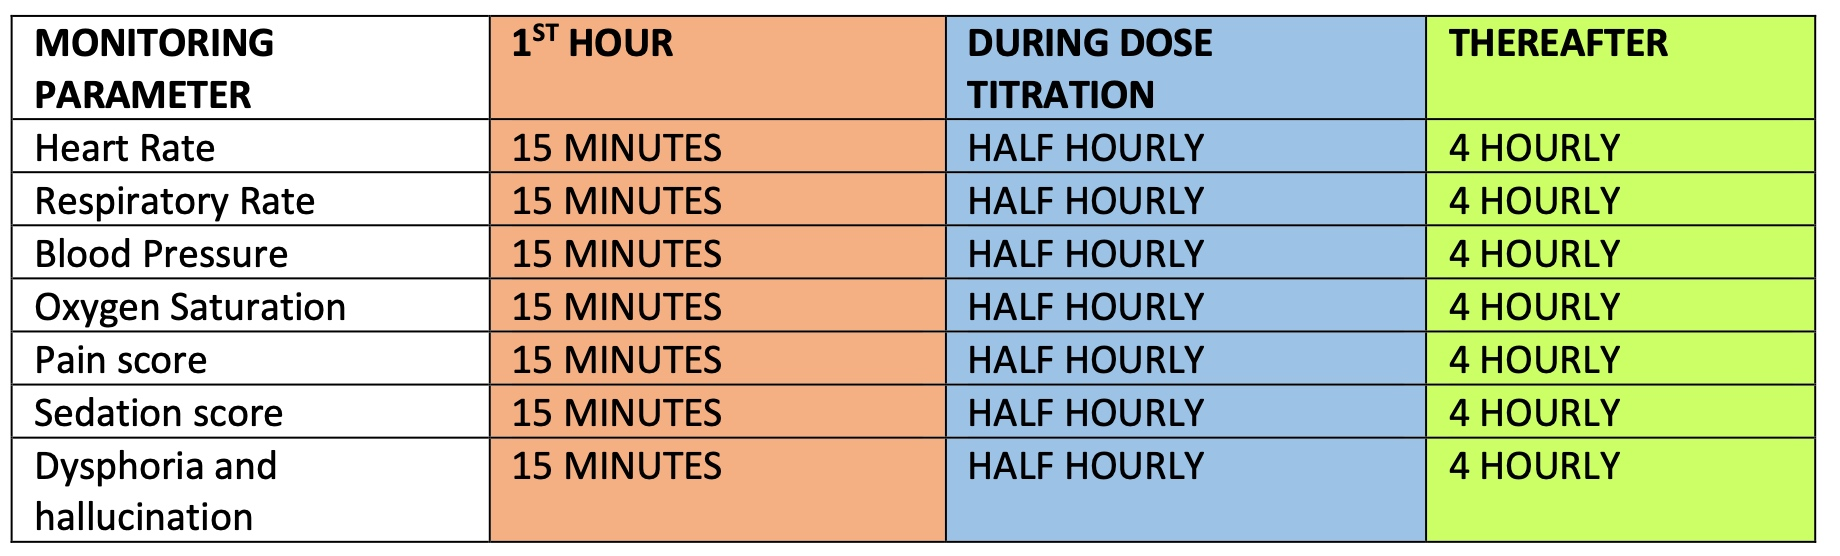
\includegraphics[width=0.7\linewidth]{pdf_monitor} \caption{Suggested frequency that a patient's observations should be recorded when starting or changing ketamine.}\label{fig:nice-fig}
\end{figure}

\hypertarget{side-effects}{%
\chapter{Side effects}\label{side-effects}}

Research has shown in low doses ketamine, the majority of people experience either mild or an absence of adverse effects. Unlike opioids, hypotension and respiratory depression are not common side effects associated with Ketamine, due to its positive inotropic effect, and ability to preserve respiratory drive. However, the most common side effects associated with ketamine are dysphoria and hallucinations.

\hypertarget{sedation}{%
\section{Sedation}\label{sedation}}

If sedation score of 2 or more or patient unarousable, stop the ketamine infusion and any opioid medications, get immediate help and administer oxygen therapy. Naloxone does not have any effect on ketamine, however it should be considered if the patient is receiving any concurrent opioids and has sedation score of 2 and/or has respiratory depression. If sedation score is 1, the infusion rate should be reduced by half. If the patient is receiving oral ketamine, to omit the next dose and request a member of the pain service to review the dosage and reassess analgesia.

\hypertarget{respiratory-depression}{%
\section{Respiratory Depression}\label{respiratory-depression}}

This is usually associated with rapid IV bolus's of ketamine, however if in the event, discontinue the infusion if respiratory rate is below 8 breaths/ minute. Discontinue any other concurrent opioids, administer oxygen therapy and get immediate help.

\hypertarget{dysphoria-hallucinations-vivid-dreams}{%
\section{Dysphoria, Hallucinations, Vivid Dreams}\label{dysphoria-hallucinations-vivid-dreams}}

Ketamine can cause a dissociative effect and can lead to dysphoria and hallucinations, however at sub-anaesthetic doses this should be rare. In the event of a patient experiencing this, please reassure the patient, and depending on the severity; either reduce the rate by half or pause infusion for one hour and re assess. If the patient is receiving oral ketamine, to omit the next dose and request a member of the pain service to review the dosage.

\hypertarget{stopping-low-dose-ketamine}{%
\chapter{Stopping Low-dose Ketamine}\label{stopping-low-dose-ketamine}}

IV and oral low-dose ketamine should be used short term when managing acute pain, usually for 72-96 hours. Patients receiving low dose ketamine will be reviewed daily by the acute pain team and any concerns should be escalated to the on-call anaesthetist out of hours.\\
Ketamine can be discontinued abruptly, as ketamine is not addictive when used short termly, and should not cause any physical or mental withdrawal symptoms. However, it can titrated down to ensure the patient does not experience a sudden return of pain. It would also be advisable to discontinue strong opioids prior to the discontinuation of ketamine, as patient can experience rebound hyper anelgesia.

  \bibliography{book.bib,packages.bib}

\end{document}
